\documentclass[12pt]{article}

\usepackage[paperheight=1.75in,paperwidth=4in,top=.25in,bottom=0in,right=0in,left=0in]{geometry}
%fancy math symbols
\usepackage{amsmath}
\usepackage{amssymb}
%DAGs
\usepackage{tikz}
\usetikzlibrary{arrows,positioning,snakes,calc,shapes}
\tikzset{>=latex}
\usepackage{float}

\begin{document}  \begin{figure}[H]    \begin{center}         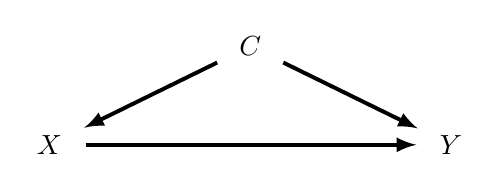
\begin{tikzpicture}        \node [align=center] (c) at (0,1.25) {$C$};    \node [align=center] (x) at (-2.55,0) {$X$};    \node [align=center] (y) at (2.55,0) {$Y$};        \begin{scope}[line width=.05cm,shorten >= 5pt, shorten <= 5pt]    \draw[->,color=black] (c) to (x);    \draw[->,color=black] (c) to (y);    \draw[->,color=black] (x) to (y);    \end{scope}        \end{tikzpicture}    \end{center}  \end{figure}\end{document}
